\section{Decision interface and model structure}
\begin{figure}[t]
\centering
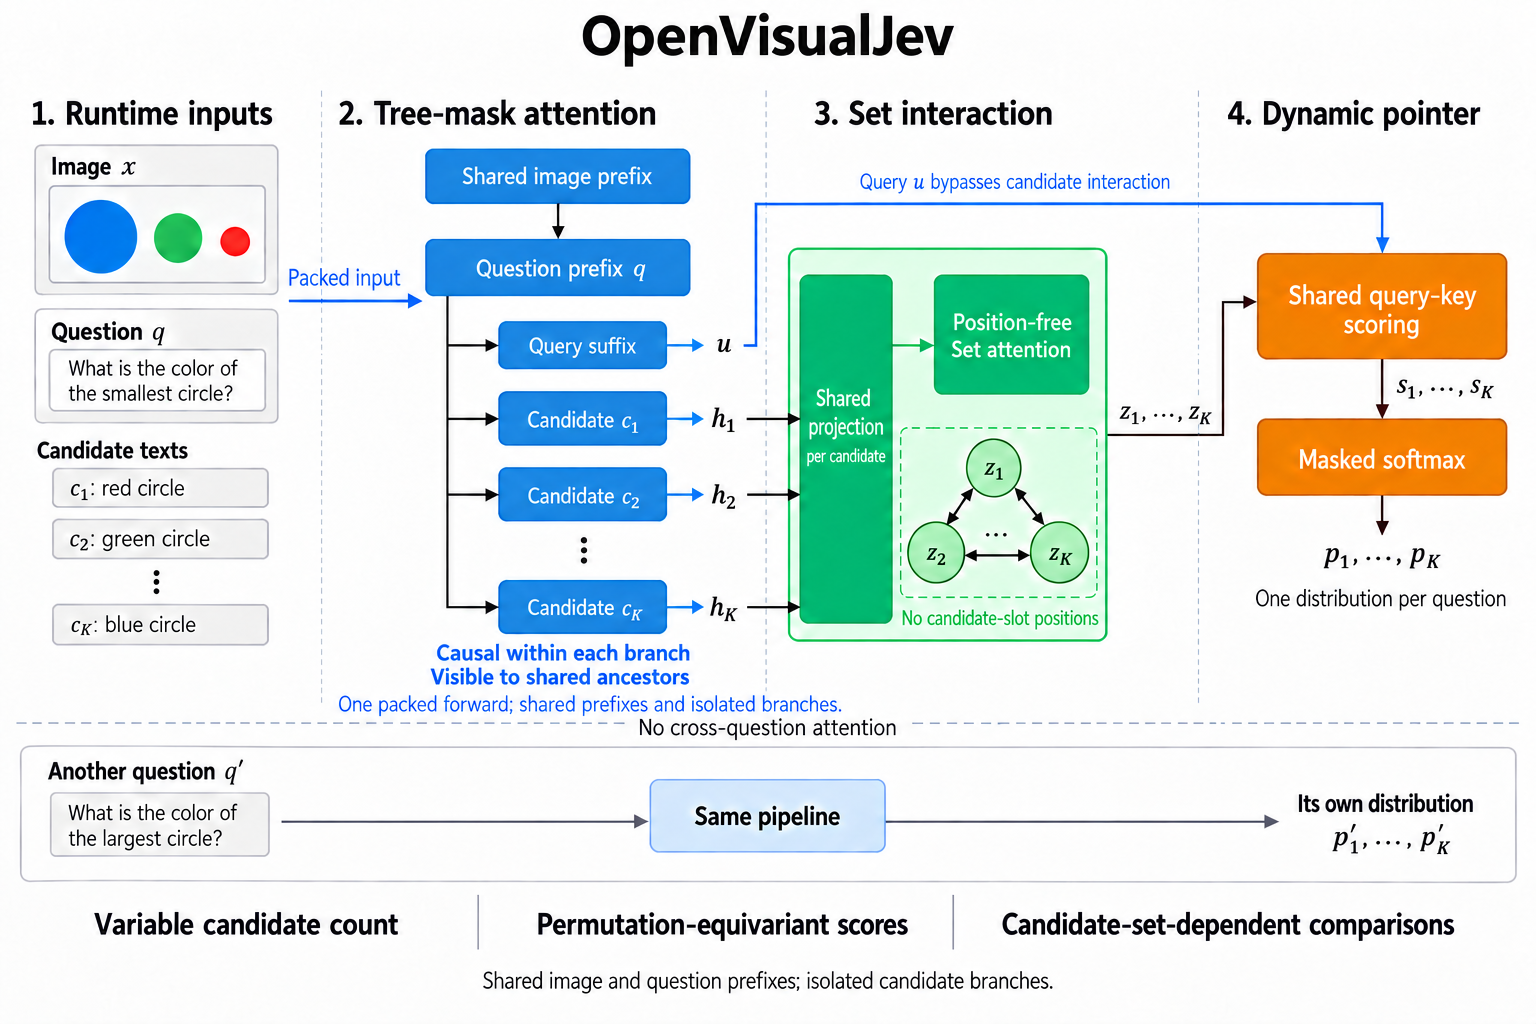
\includegraphics[width=\linewidth]{../figures/set-pointer-method.png}
\caption{OpenVisualJev. Tree-masked attention shares image and question prefixes across isolated query and candidate suffixes. Tokens attend to causal predecessors and ancestors. Position-free Set attention compares candidate representations; the query bypasses this module and scores its outputs through a shared pointer. Interaction and normalization are question-local. Training-time confidence regularization and held-out temperature scaling calibrate the output probabilities.}
\label{fig:set-pointer-method}
\end{figure}

Given an image $x$, a question $q$, and runtime candidate texts $C=(c_i)_{i=1}^{K}$, OpenVisualJev returns a normalized distribution over mutually exclusive candidate slots. External identifiers associate outputs with inputs; prompts contain image, question, and candidate content.

\subsection{Tree-masked multimodal encoding}
The input tree contains a shared image prefix, one prefix per question, and separate query and candidate suffixes. Each prefix appears once. Tokens attend to causal predecessors within their segment and to ancestors; sibling candidates and different questions remain isolated.

\paragraph{Visibility and positions.}
Let $\mathcal A(t)$ contain tokens in the ancestor segments of token $t$, and let $\mathcal C(t)$ contain tokens up to and including $t$ within its own segment. The binary visibility mask is $M_{ts}=\mathrm{I}[s\in\mathcal A(t)\cup\mathcal C(t)]$.
The shared root is causal; a question prefix reads the root and its own history; each leaf additionally reads its question prefix. Masked entries are excluded from attention normalization. Packed offsets only locate tokens in memory: multimodal position coordinates follow the original root-to-leaf sequence. Consequently, placing one candidate before another in the packed sequence creates no additional attention edge between them.

\paragraph{Branch representations.}
Let $E_\theta$ return the final valid-token representation along a root-to-leaf path. The query yields $u=E_\theta(x,q)$, and candidate $i$ yields $h_i=E_\theta(x,q\mathbin{\Vert}\texttt{Candidate:}\mathbin{\Vert}c_i)$. One packed forward computes all leaves, injecting visual features at the shared root. Original branch-local multimodal positions preserve each candidate's coordinates and visible context under reordering.

For multiple questions about one image, each question receives its own internal prefix and leaf group beneath the shared root. Final-token representations are gathered by leaf identity and passed to separate question-local scoring operations. Adding another question therefore adds a disjoint subtree while retaining the existing questions' visible tokens. Candidate count determines the number of leaves and the size of the subsequent set operation; the encoder and pointer parameters are shared across counts.

\subsection{Set interaction and dynamic pointer}
\paragraph{Position-free candidate interaction.}
Stacking candidate representations as rows of $H$, we apply a shared projection and position-free self-attention module $S_\phi$. The query bypasses this module. Scores and probabilities are
\begin{equation}
 Z=S_\phi(H),\qquad s_i=\frac{\langle W_q\operatorname{LN}(u), W_k\operatorname{LN}(Z_i)\rangle}{\sqrt{d}},\qquad p_i=\frac{\exp(s_i)}{\sum_{j\in\mathcal V}\exp(s_j)},
\end{equation}
where $d$ is the query--key dimension and $\mathcal V$ indexes valid slots. Padding is excluded from attention and probability normalization.

\subsection{Structural properties}
\paragraph{Permutation-equivariant scoring.}
Shared row-wise operations commute with a candidate permutation $P$. Consistently permuting query, key, value, and mask gives $\operatorname{Attn}(PH)=P\operatorname{Attn}(H)$; residuals and row-wise normalization preserve this relation. Thus $s(PH)=Ps(H)$ and $p(PH)=Pp(H)$ in exact arithmetic, provided branch preprocessing and positions are unchanged and candidate indices are omitted.

With a unique maximum, the selected candidate identity is preserved under candidate reordering.

The attention relation follows from permuting both axes of the attention matrix: if $A=\operatorname{softmax}(QK^\top/\sqrt d)$, then the permuted matrix is $PAP^\top$. Multiplication by the permuted values $PV$ gives $PAV$. This identity extends through each candidate block, while the shared query remains unchanged. The pointer therefore permutes output slots together with their candidate identities.

\paragraph{Question isolation and candidate-set dependence.}
Tree masking isolates questions, and Set attention and normalization operate within each question. Within a question, logits depend on all candidates, so $p_i/p_j=\exp(s_i-s_j)$ can change when the candidate set changes.

\subsection{Training and probability calibration}
\paragraph{Calibration-aware training.}
We augment cross-entropy with dataset-wise confidence--accuracy alignment, following DCA~\citep{liang_2020_dca}. For dataset groups $B(d)$ in an effective batch, define $a_n=\arg\max_i p_{n,i}$, confidence $c_n=\max_i p_{n,i}$, and correctness $r_n=\mathrm{I}[a_n=y_n]$. Over represented datasets $\mathcal D$, we optimize
\begin{equation}
\begin{aligned}
\mathcal L_{\mathrm{train}}&=\mathcal L_{\mathrm{CE}}+\lambda\mathcal L_{\mathrm{conf}},\\
\mathcal L_{\mathrm{conf}}&=\frac{1}{|\mathcal D|}\sum_{d\in\mathcal D}
\left[\frac{1}{|B(d)|}\sum_{n\in B(d)}\left(c_n-\operatorname{stopgrad}(r_n)\right)\right]^2.
\end{aligned}
\label{eq:training-objective}
\end{equation} Balanced batches weight datasets equally. Gradients flow through confidence while correctness is detached. The loss ablation sets $\lambda=0$ under matched sampling and optimization.

The two loss terms operate at different levels. Cross-entropy supervises each target candidate, whereas the confidence term aligns mean confidence and accuracy within each dataset. Equal group weighting prevents datasets with more examples in an effective batch from dominating that alignment. Post-training temperature fitting then adjusts the frozen model's probability scale on a separate data split.

\paragraph{Reserved probability calibration.}
With model weights frozen, we fit $T>0$ on reserved calibration data by minimizing candidate-event NLL. Predictions use $p_i^{(T)}=\exp(s_i/T)/\sum_{j\in\mathcal V}\exp(s_j/T)$. Scalar scaling preserves ranking, candidate identity, and permutation equivariance.
